\documentclass[a4j,titlepage]{jarticle}
\usepackage[dvipdfmx]{graphicx}
\usepackage{ascmac}
\usepackage{float}
\usepackage{amssymb}%にやりイコールを使う
\usepackage{multirow}
\usepackage{multicol}
\usepackage{tabularx}
%\usepackage{color}

\begin{document}

\title{2022 年度 3 回生前期学生実験 HW  \\ \bf team02 機能設計仕様書 植田健斗担当分}
% ↓ここに自分の氏名を記入
\author{機能設計仕様書作成者:植田健斗\\
グループメンバー:\\伊藤舜一郎 (学籍番号:1029-32-7548)
\\植田健斗 (学籍番号:1029-32-6498)}
\西暦
\date{提出期限:6月9日13時 提出日: \today} % コンパイル時の日付が自動で挿入される
\maketitle
\newpage


\section{全体のコンポーネント分割方法}

%\subsection{設計する回路の仕様}
%\subsection{設計の詳細}
%\subsubsection{ピン割当て}
%\subsection{正しく動作したか}
それぞれの機能を持った回路ごとにモジュール分割した。
各回路につけたファイル名は図\ref{moduleSplit0422}に示した通りである。


\begin{figure}[H]
    \begin{center}
    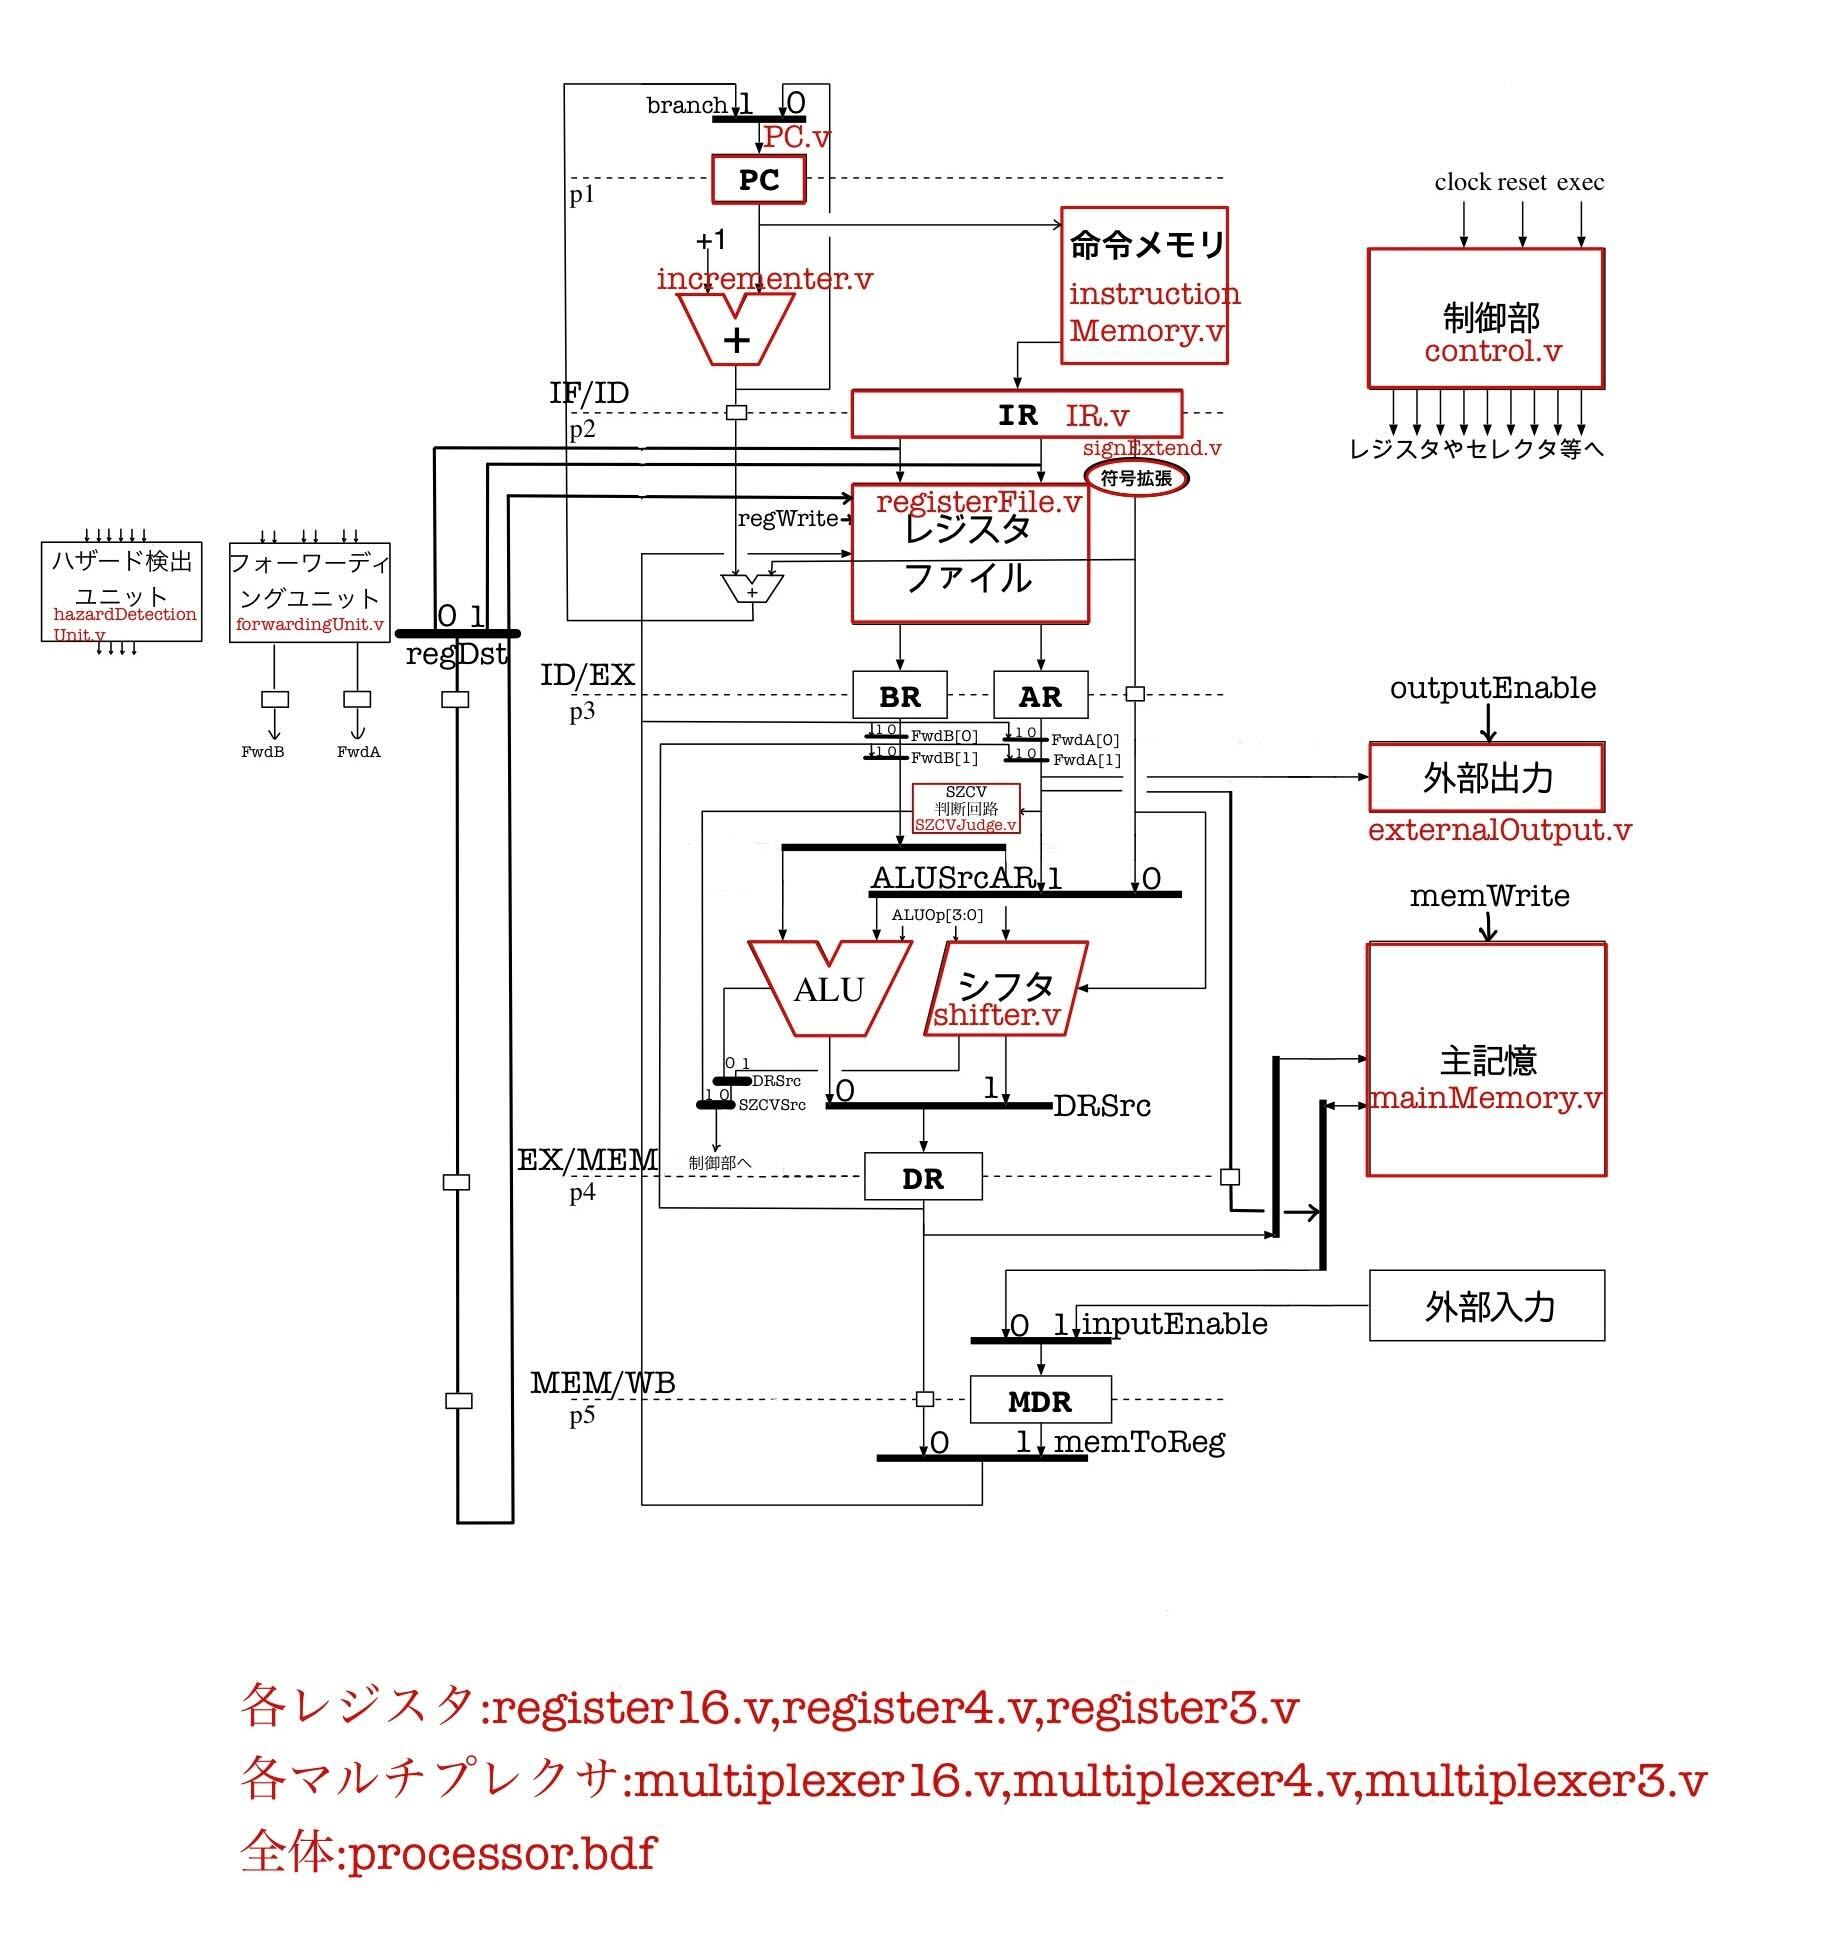
\includegraphics[scale = 0.22]{structure0530.jpg}
    \end{center}
    \caption{コンポーネント分割の方法の図}
    \label{moduleSplit0422}
\end{figure}

追加・変更したコンポーネントの役割分担の表を以下の表\ref{rolesDivision0422}に示す。

\begin{table}[H]
    \caption{役割分担(最終報告時点)}
    \label{rolesDivision0422}
    \begin{center}
    \begin {tabular}{|c|c|c|} \hline
         コンポーネント & 追加か変更か & 担当 \\ \hline \hline
         フォーワーディングユニット & 追加 & 伊藤\\ \hline
         クロックカウンター & 追加 & 伊藤 \\ \hline
         アセンブリコード(基数ソート) & (応用プログラム) & 伊藤\\ \hline
         ハザード検出ユニット & 追加 & 植田\\ \hline
         パイプラインレジスタ & 追加 & 植田\\ \hline
         命令メモリ & 追加 & 植田 \\ \hline
         制御部 & 変更 & 植田\\ \hline
         レジスタファイル & 変更 & 植田 \\ \hline
         全体 & 変更 & 植田 \\ \hline
         アセンブリコード(度数ソート) & (ソートコンテスト用) & 植田(レポートは伊藤) \\ \hline
    \end {tabular}
    \end{center}
\end{table}




\newpage
\section{変更を加えたコンポーネント}
\subsection{レジスタファイル(registerFile.v)}

\subsubsection{外部仕様 入力}
この回路の入力は以下の表\ref{registerFileI}のようになる。
\begin{table}[H]
    \caption{レジスタファイル(registerFile.v)の入力(=input)}
    \label{registerFileI}
    \begin{center}
    \begin {tabularx}{150mm}{|c|X|} \hline
         input & inputの説明 \\ \hline \hline
         Rs[2:0] & 命令中のRs・Raフィールドを受け取る。\\ \hline
         Rd[2:0] & 命令中のRd・Rbフィールドを受け取る。\\ \hline
         regWrite & 内部のレジスタが書き換え可能かを表す信号 regWriteとchangeEnableがともに1のときのみ書き換え可能\\ \hline
         writeData[15:0] & レジスタに書き込むデータ\\ \hline
         writeRegister[2:0] & writeData[15:0]を書きこむレジスタの番号\\ \hline
         clock & クロック信号。clockの立ち上がりで、レジスタ書きこみが可能な場合、書きこみが行われる。\\ \hline
         reset & 初期化信号。resetが1のときにクロックが立ち上がると、レジスタの中身を0で初期化する。\\ \hline
         changeEnable & 内部のレジスタが書き換え可能かを表す信号。regWriteとchangeEnableがともに1のときのみ書き換え可能\\ \hline
    \end{tabularx}
    \end{center}
\end{table}

\subsubsection{外部仕様 出力}
この回路の出力は以下の表\ref{registerFileO}のようになる。
\begin{table}[H]
    \caption{レジスタファイル(registerFile.v)の出力(=output)}
    \label{registerFileO}
    \begin{center}
    \begin {tabularx}{150mm}{|c|X|} \hline
         output & outputの説明 \\ \hline \hline
         AR[15:0] & Rs(Ra)フィールドで指定したレジスタに格納されているデータを読み込む。 \\ \hline
         BR[15:0] & Rd(Rb)フィールドで指定したレジスタに格納されているデータを読み込む。 \\ \hline
    \end {tabularx}
    \end{center}
\end{table}

\subsubsection{内部仕様}
内部に8個の16bitレジスタreg [15:0] r [7:0]を持ち、
入力Rs[2:0],Rd[2:0]の値に応じたレジスタに格納されたデータを
それぞれAR[15:0],BR[15:0]として出力する。

また、resetが0でchangeEnableとregWriteがともに1のときのみ書き換え可能状態になり、
この状態でclockが立ち上がると、入力writeData[15:0]で受け取ったデータを
writeRegister[2:0]に対応する番号の内部レジスタrにデータを書きこむ。

regWriteが1のときに、writeRegister[2:0]とRs[2:0]もしくはRd[2:0]の値が等しいときは
AR[15:0]もしくはBR[15:0]には、writeData[15:0]が出力される。

resetが1のときにclockが立ち上がると、
すべての内部レジスタrの値を0で初期化する。

このレジスタファイルはレジスタへの書き込みとそのレジスタからのデータの読み出しを
同じクロック周期の中で行ったときに、
中間報告時点で作成したレジスタファイルでは、
書き込みを行う前のデータが読みだされてしまっていたが、
最終報告の段階では
あるレジスタへの書き込みとそのレジスタからのデータの読み出しを
同じクロック周期の中で行ったときに、
同じクロックの中で書き込みするデータを読みだせるように
改良をした。






\newpage
\subsection{制御部(control.v)}

\subsubsection{外部仕様 入力}
この回路の入力は以下の表\ref{controlI}のようになる。
\begin{table}[H]
    \caption{制御部(control.v)の入力(=input)}
    \label{controlI}
    \begin{center}
    \begin {tabularx}{150mm}{|c|X|} \hline
         input & inputの説明 \\ \hline \hline
         clock & クロック信号。clock立ち上がりで、レジスタ書きこみが可能な場合、書きこみが行われる。 \\ \hline 
         instruction[15:0] & 命令の格納されたIRの出力を受け取る。 \\ \hline 
         reset & 初期化信号。resetが1のときにクロックが立ち上がると、出力systemRunning信号を0にする。 \\ \hline
         exec & 全体の実行・停止信号execを受け取る。\\ \hline
         SZCV[3:0] & 前回の命令でのSZCVフラグを受け取る。LD,IN命令のときはSZCVの値は未定義\\ \hline
    \end{tabularx}
    \end{center}
\end{table}

\subsubsection{外部仕様 出力}
この回路の出力は以下の表\ref{controlO}のようになる。
\begin{table}[H]
    \caption{制御部(control.v)の出力(=output)}
    \label{controlO}
    \begin{center}
    \begin {tabularx}{150mm}{|c|X|} \hline
         output & outputの説明 \\ \hline \hline
         regDst & 書き込みをするレジスタを、入力Instruction[10:8](Rd,Rbフィールド)で指定する(=0)か、Instruction[13:11](Ra,Rsフィールド)で指定する(=1)かを決める。\\ \hline %%%%%
         ALUSrcAR & ALUの入力inB[15:0]の受け取る値が、命令中の即値(=0)か、ARの値(=1)かを決める。\\ \hline
         ALUOp[3:0] & ALUの入力op[3:0]に入力する値で、ALUで行う演算を決める。\\ \hline
         DRSrc & DRに入力する値を、ALUの出力out[15:0]にする(=0)か、シフタの出力out[15:0]にする(=1)かを決める。
         また、SZCVに入力する値を、ALUの出力SZCV[3:0]にする(=0)か、シフタの出力SZCV[3:0]にする(=1)かを決める。\\ \hline
         outputEnable & 外部出力に値を受け渡す(=1)か受け渡さない(=0)かを決める。正確にはOUT命令のときのみ1となる。\\ \hline
         SZCVSrc & SZCVフラグをALU・シフタの値をもとに決めるか(=0)、ARの値をもとに決める(=1)かを決める。\\ \hline
         memRead & LD命令とIN命令の時に1になる。そのほかは0になる。\\ \hline
         inputEnable & 外部入力から値を受け取る(=1)か受け取らない(=0)かを決める。正確にはIN命令のときのみ1となる。\\ \hline
         memWrite & メモリに書きこむ(=1)か書きこまない(=0)かを決める。正確にはST命令のときのみ1となる。\\ \hline
         branch & 入力のSZCV[3:0]とinstruction[15:0]から、分岐をする(=1)か、分岐をしない(=0)かを決める。\\ \hline
         regWrite & レジスタファイルに書き込みを行う(=1)か、レジスタファイルに書き込みを行わない(=0)かを決める。\\ \hline
         memToReg & プログラムカウンタや、レジスタファイルに渡すデータを、DRの値にする(=0)かMDRの値にする(=1)かを決める。\\ \hline
         notReadRsRd & IDフェーズでデコードした命令がNOP,HLT,LI,B,BE,BLT,BLE,BNEのときに1になり、パイプラインストールを起こさない。それ以外のときは0\\ \hline
         systemRunning & すべてのレジスタの書き換えを不可能にする(=0)か可能にする(=1)かを決める。
         つまり、機械が実行待機状態(=0)か動作状態(=1)かを決める。\\ \hline
         IFFlush & 通常は0で、HLT命令がIDフェーズで処理された時から、そのHLT命令がWBフェーズにある時まで、1になる。\\ \hline
         PCWrite & 通常は1で、HLT命令がIDフェーズで処理された時から、そのHLT命令がWBフェーズにある時まで、0になる。\\ \hline
    \end {tabularx}
    \end{center}
\end{table}

\subsubsection{内部仕様}
systemRunningという1bitの内部レジスタを持ち、
その値を変えることで機械を実行待機状態(systemRunning=0)か実行状態(systemRunning=1)かを
切り替えている。
exec入力については1クロック前のexec入力を保持する1bitレジスタexec\_preと
カウンタを表す16bitの内部レジスタcounterを
持つ。これを用いて以下の表\ref{execexecprecntsystemRunningRelation}のようにexecとexec\_preの値に応じて、
counterとsystemRunningを変更する。これによりexecボタンのチャタリングを除去しながら、
execボタンが押されるたびに
機器が実行状態かどうかを決めるsystemRunningを反転させることができる。


\begin{table}[H]
    \caption{execとexec\_preとcnt(=counter)の値に応じて、更新するcnt(=counter)とsystemRunningの値}
    \label{execexecprecntsystemRunningRelation}
    \begin{center}
    \begin {tabularx}{145mm}{|c||cccX|} \hline
         exec\_pre exec & 00 & 01 & 10 & 11 \\ \hline \hline
         cnt=0 & cnt\textless =0 & cnt\textless =1 & cnt\textless =1 & cnt\textless =0 \\ \hline
         0\textless cnt\textless 15 & cnt\textless =cnt+1 & cnt\textless =0 & cnt\textless =0 & cnt\textless =cnt+1 \\ \hline
         cnt=15 & cnt\textless =0 & cnt\textless =0 & cnt\textless =0 & cnt\textless =0,              sysstemRunning\textless =$\sim$sysstemRunning \\ \hline 

    \end {tabularx}
    \end{center}
\end{table}

resetが呼ばれると、
\begin{verbatim} 
    counter <= 16'h 0000;
    systemRunning <= 1'b 0;
    exec\_pre <= exec;
\end{verbatim}
により初期化を行う。
resetが押されるとsystemRunningは0になるので、
実行が停止し、実行待機状態になる。その後execボタンが押されることで
systemRunningが1になり実行が行われるようになる。
また、インプット命令のEXフェーズと
halt命令のWBフェーズでsystemRunningを0にし
実行待機状態になるようにしている。
この場合もexecボタンを押すことで実行を再開できる。

HLT命令の処理は以下の図\ref{haltsiyuo}ように行っている。

\begin{figure}[H]
    \begin{center}
    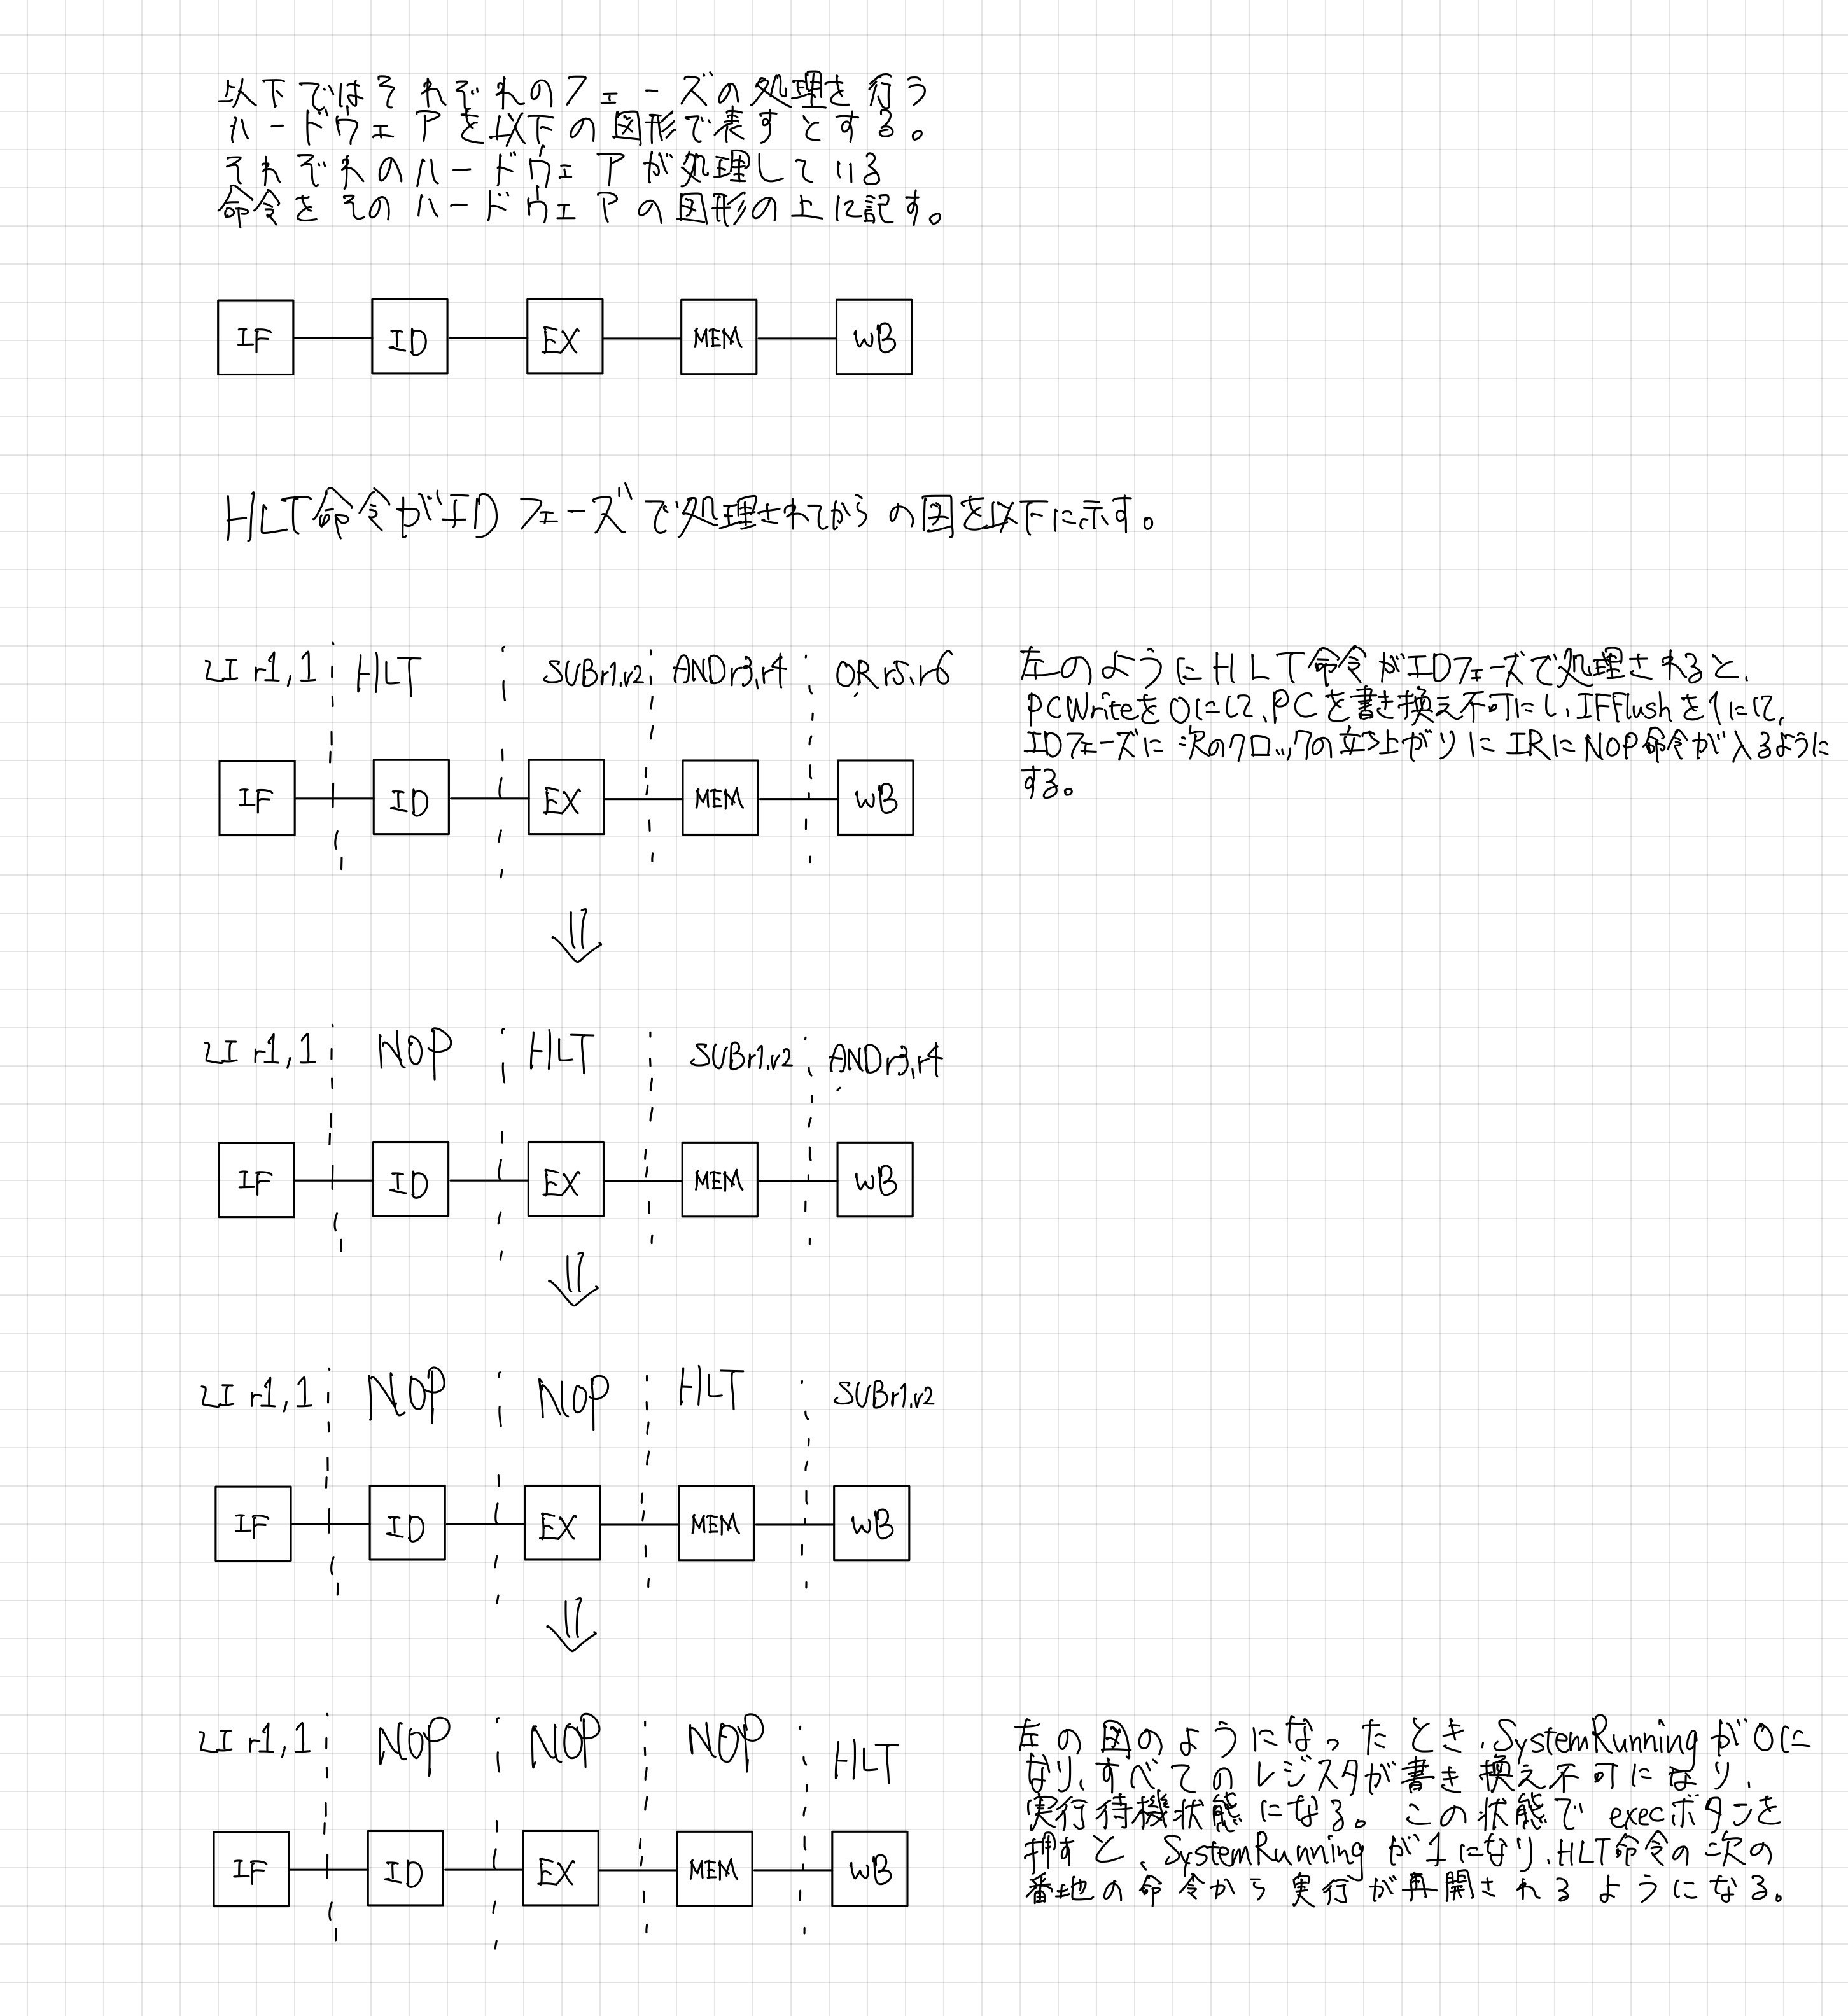
\includegraphics[scale = 0.22]{haltnosiyou.jpg}
    \end{center}
    \caption{HLT命令が呼ばれたときの制御}
    \label{haltsiyuo}
\end{figure}


各制御信号は組み合わせ回路を用いて実現している。
以下の表\ref{controlsignal}でそれぞれの制御信号の出力の仕様をまとめた。


\begin{table}[H]
    \caption{制御信号の仕様}
    \label{controlsignal}
    \begin{center}
    \begin{tabularx}{150mm}{|c|X|} \hline
         制御信号名 & 制御信号の仕様 \\ \hline \hline
         regDst & LD命令の時のみ1 \\ \hline %%%%%
         ALUSrcAR & 演算,シフト,IN,OUT,NOP,HALT命令の時に1になる。(MOVの下のreservedの時も1) \\ \hline
         ALUOp[3:0] & 演算命令(MOVの下のreservedも含む)のときはinstruction[7:4](命令で指定した演算)になる。LI命令の時は4'b 0110(MOV命令)になる。その他のときは4'b 0000(アドレス計算のための足し算)になる。 \\ \hline
         DRSrc & シフト,IN,OUT,NOP,HALT命令の時のみ1  \\ \hline
         outputEnable & OUT命令の時のみ1  \\ \hline
         SZCVSrc & 演算、シフト、IN,OUT,NOP,HALT,LD,ST命令の時に1になる。(MOVの下のreservedの時も1) \\ \hline
         memRead & IN,LD命令のときのみ1になる。LD,IN命令のときに入力されるデータを次の命令で読み出す際におこるデータハザードが起こるかどうか判定する。 \\ \hline
         inputEnable & IN命令の時のみ1  \\ \hline
         memWrite & ST命令の時のみ1  \\ \hline
         branch & B命令または(BE命令かつZ=1)または(BLT命令かつS\textasciicircum V=1)または(BLE命令かつZ\textbar (S\textasciicircum V)=1)または(BNEかつ$\sim$Z=1)のときのみ1  \\ \hline
         regWrite & ADD,SUB,AND,OR,XOR,MOV,シフト,IN,LD,LI命令の時のみ1 \\ \hline
         memToReg & LD,IN命令の時のみ1 \\ \hline
         notReadRsRd & NOP,HLT,B,BE,BLT,BLE,BNEのとき1となる。これが1のとき、パイプラインストールストールを起こさない。  \\ \hline
         IFFlush & 通常は0でHLT命令がIDフェーズで読み込まれたときから、4サイクルの間、IFFlushは1になる。
         HLT命令以降の命令で読み込まれたものを実行しないようにNOP命令に置き換える。  \\ \hline
         PCWrite & 通常は1でHLT命令がIDフェーズで読み込まれたときから、4サイクルの間、PCWriteは0になる。
         HLT命令がIDフェーズに来た時にPCを書き換え不可にし、HLT命令がある次の番地にPCの値を固定する。  \\ \hline
    \end{tabularx}
    \end{center}
\end{table}


%%%%%%%%%%%%%%%%%%%%%%%%%%%


\newpage
\section{追加したコンポーネント}
\subsection{ハザード検出ユニット(hazardDetectionUnit.v)}
パイプラインハザードとは
、ここではLD,IN命令の直後の命令でLD,IN命令により保存したデータを参照することによるデータハザードを指している。

\subsubsection{外部仕様 入力}
この回路の入力は以下の表\ref{hazardDetectionUnitI}のようになる。
\begin{table}[H]
    \caption{ハザード検出ユニット(hazardDetectionUnit.v)の入力(=input)}
    \label{hazardDetectionUnitI}
    \begin{center}
    \begin {tabularx}{150mm}{|c|X|} \hline
         input & inputの説明 \\ \hline \hline
         IDEX\_memRead & EXフェーズで処理をしている命令のmemRead信号を受け取る。\\ \hline
         IDEX\_RegRd[2:0] & EXフェーズで処理をしている命令の書き込みレジスタの番号を受け取る。\\ \hline
         IFID\_Rs[2:0] & IDフェーズで処理している命令中のRsフィールドの値を受け取る。\\ \hline
         IFID\_Rd[2:0] & IDフェーズで処理している命令中のRdフィールドの値を受け取る。\\ \hline
         notReadRsRd & 制御部(control.v)の出力notReadRsRdを受け取る。\\ \hline
         branch & 制御部(control.v)の出力branchを受け取る。\\ \hline
    \end{tabularx}
    \end{center}
\end{table}

\subsubsection{外部仕様 出力}
この回路の出力は以下の表\ref{hazardDetectionUnitO}のようになる。パイプラインハザードとは
、ここではLD,IN命令の直後の命令でLD,IN命令により保存したデータを参照することによるデータハザードを指している。
\begin{table}[H]
    \caption{ハザード検出ユニット(hazardDetectionUnit.v)の出力(=output)}
    \label{hazardDetectionUnitO}
    \begin{center}
    \begin {tabularx}{150mm}{|c|X|} \hline
         output & outputの説明 \\ \hline \hline
         PCWrite & パイプラインハザードが起きた時に0になり、PCの書き換えをやめる。 \\ \hline
         IFIDWrite & パイプラインハザードが起きた時に0になり、IFフェーズとIDフェーズの間のパイプラインレジスタ(IR)の書き換えをやめる。 \\ \hline
         IFFlush & 分岐が成立したときに1になり(=branch)、IRにPCのアドレスで命令メモリから読み出した命令ではなく、NOP命令を入力する。\\ \hline
         IDFlush & パイプラインハザードが起きた時に1になり、IDフェーズとEXフェーズの間にある制御信号が格納されたパイプラインレジスタの値を初期化する。\\ \hline
    \end {tabularx}
    \end{center}
\end{table}

\subsubsection{内部仕様}
組み合わせ回路を用いて実現されている。
LD,IN命令で読み込んだ命令を直後の命令で参照する際におこるデータハザードと、
分岐命令の際の制御ハザードに対処するために、制御信号を出す。

LD,IN命令で読み込んだ命令を直後の命令で参照する際におこるデータハザードへの対処と
分岐命令の際の制御ハザードへの対処は以下の図\ref{bunkide-ta}ように行っている。

\begin{figure}[H]
    \begin{center}
    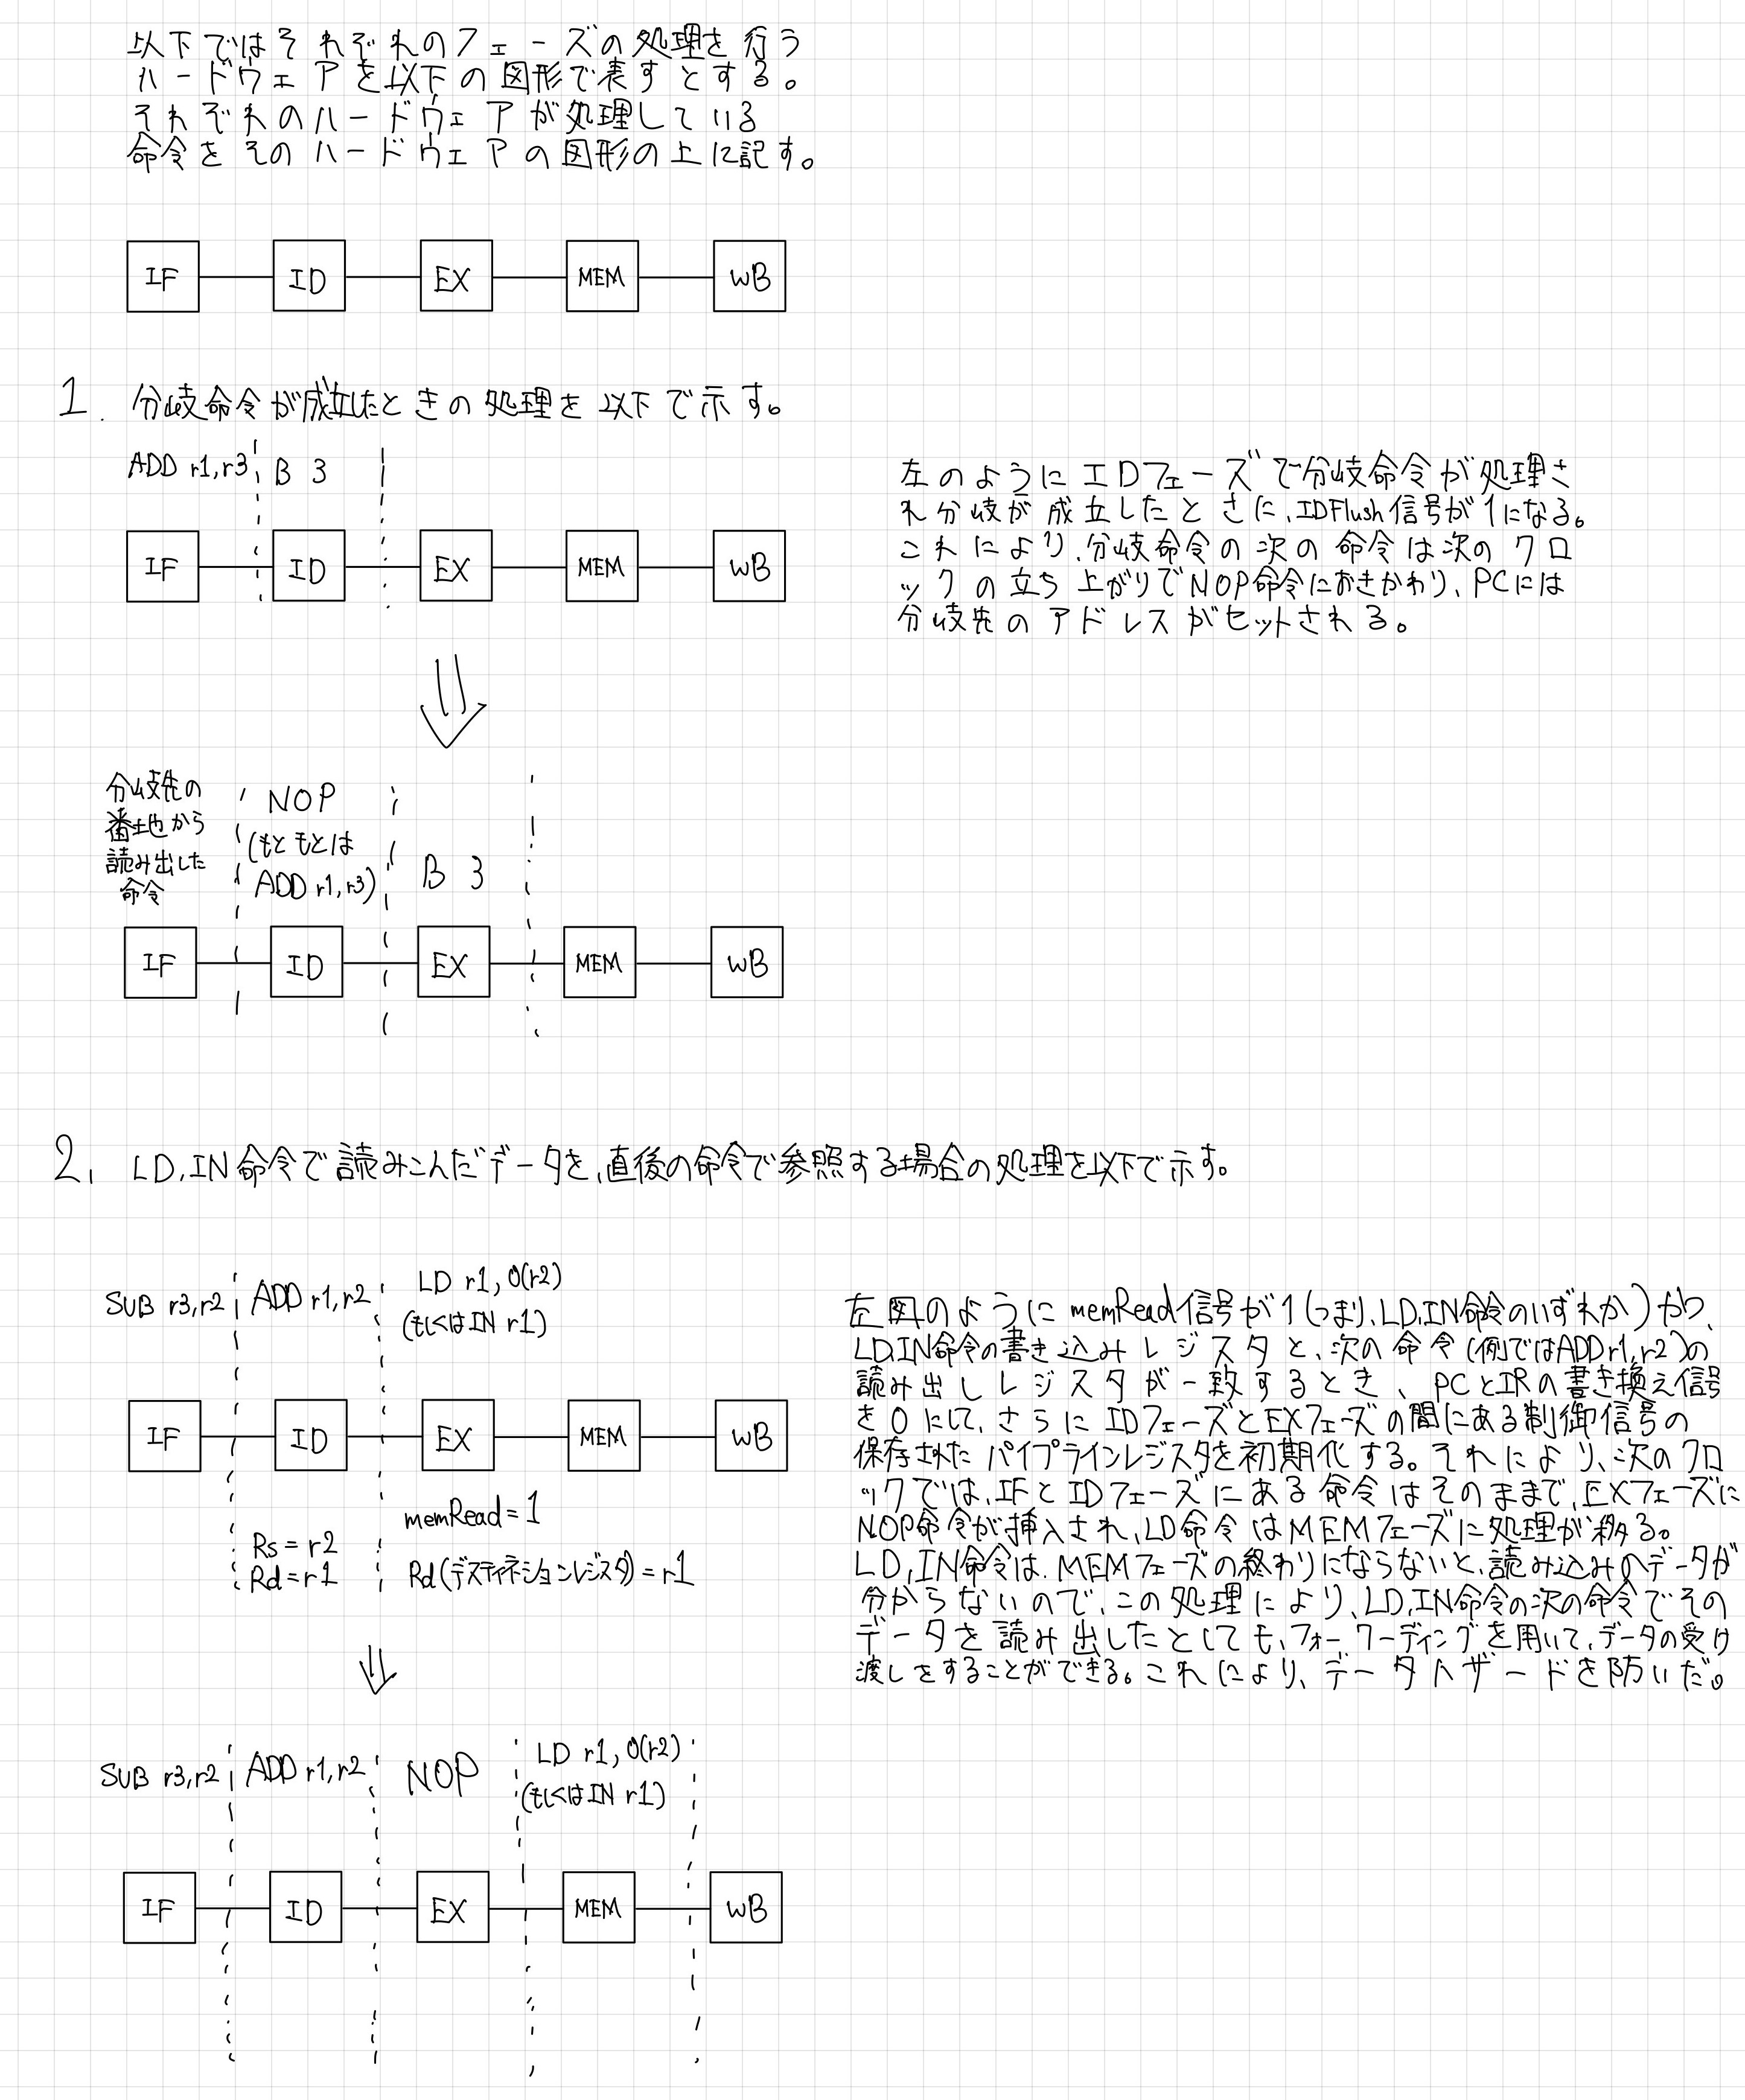
\includegraphics[scale = 0.22]{bunkidata.jpg}
    \end{center}
    \caption{分岐命令の制御ハザードと、LD,IN命令で読み込んだ命令を直後の命令で参照する際におこるデータハザードへの対処}
    \label{bunkide-ta}
\end{figure}


\newpage
\subsection{命令メモリ(instructionMemory.v)}

\subsubsection{外部仕様 入力}
この回路の入力は以下の表\ref{instructionMemoryI}のようになる。
\begin{table}[H]
    \caption{命令メモリ(instructionMemory.v)の入力(=input)}
    \label{instructionMemoryI}
    \begin{center}
    \begin {tabularx}{150mm}{|c|X|} \hline
         input & inputの説明 \\ \hline \hline
         address[11:0] & PCの値を受け取る。メモリの読み書きを行う番地のアドレス。\\ \hline
         clock & クロック信号を反転させて入力する。clockの立ち上がり(=クロック信号の立ち下り)で、メモリ書きこみが可能な場合書きこみが行われ、また、
         address[11:0]により指定した番地のデータの読み出しが行われる。 \\ \hline 
         data[15:0] & メモリに書きこむためのデータ。このメモリには書き込みは行われない。\\ \hline
         wren & 書き込み可能信号。常に0が入力される。\\ \hline
    \end{tabularx}
    \end{center}
\end{table}

\subsubsection{外部仕様 出力}
この回路の出力は以下の表\ref{instructionMemoryO}のようになる。
\begin{table}[H]
    \caption{命令メモリ(instructionMemory.v)の出力(=output)}
    \label{instructionMemoryO}
    \begin{center}
    \begin {tabularx}{150mm}{|c|X|} \hline
         output & outputの説明 \\ \hline \hline
         q[15:0] & メモリから読み出しされたデータ\\ \hline
    \end {tabularx}
    \end{center}
\end{table}

\subsubsection{内部仕様}
RAMを用いて実装した。PCの下位12bitであるaddress[11:0]で指定した番地に対して、
clockが立ち上がる度にデータの読み出しを行う。
書き込みは行われない。
ROMでの実装でも良いが拡張する可能性を考えてRAMでの実装にしている。

命令を格納するためのメモリである。
dosuSort.mifをここにセットし、ソートするデータが0x400から0x7ff番地に書かれたmifファイル(sorted.mif,random.mif,r\_sorted.mif)をmainMemory.vに入れることで、度数ソートを実行できる。

%%%%%%%%%%%%%%%%%%%%%%%%%%%

\newpage
\subsection{パイプラインレジスタ(IDEXRegister.v,EXMEMRegister.v,MEMWBRegister.v)}

\subsubsection{外部仕様 入力}
この回路の入力は以下の表\ref{pipelineRegisterI}のようになる。
\begin{table}[H]
    \caption{パイプラインレジスタ(IDEXRegister.v,EXMEMRegister.v,MEMWBRegister.v)の入力(=input)}
    \label{pipelineRegisterI}
    \begin{center}
    \begin {tabularx}{150mm}{|c|X|} \hline
         input & inputの説明 \\ \hline \hline
	 各制御信号 & クロックの立ち上がりにレジスタ書き込み可能ならば、内部のレジスタに書きこむ値\\ \hline
     clock & クロック信号。clockの立ち上がりで、レジスタ書きこみが可能な場合、書きこみが行われる。\\ \hline %%%%%
     changeEnable & 内部のレジスタが書き換え可能かを表す信号(イネーブル信号)。この信号が1のときにclockが立ち上がると内部のレジスタの値が更新される。 \\ \hline
     reset & 初期化信号。resetが1のときにクロックが立ち上がると、レジスタの中身を0で初期化する。\\ \hline
     IDFlush & IDEXRegister.vのみ存在。1のときにクロックが立ち上がると制御信号をすべて0にする。\\ \hline
    \end{tabularx}
    \end{center}
\end{table}

\subsubsection{外部仕様 出力}
この回路の出力は以下の表\ref{pipelineRegisterO}のようになる。
\begin{table}[H]
    \caption{パイプラインレジスタ(IDEXRegister.v,EXMEMRegister.v,MEMWBRegister.v)の出力(=output)}
    \label{pipelineRegisterO}
    \begin{center}
    \begin {tabularx}{150mm}{|c|X|} \hline
     output & outputの説明 \\ \hline \hline
	 各制御信号 & 内部のレジスタに格納されている制御信号の値を出力する。\\ \hline %%%%%
\end {tabularx}
    \end{center}
\end{table}

\subsubsection{内部仕様}
レジスタを表している。
clockの立ち上がりごとに以下のことを行う。
reset信号が1のときレジスタを0で初期化する。
reset信号が0のとき、changeEnableが1なら、
入力の制御信号の値を内部のレジスタに格納する。
それ以外ならば値の変更は何もしない。
内部レジスタの値を常に出力する。
IDEXRegister.v,EXMEMRegister.v,MEMWBRegister.vはそれぞれIDEXフェーズ間、EXMEMフェーズ間、MEMWBフェーズ間の制御信号を格納するパイプラインレジスタを
表している。

%%%%%%%%%%%%%%%%%%%%%%%%%%%


\newpage
\subsection{全体(processor.bdf)}

\subsubsection{外部仕様 入力}
この回路の入力は以下の表\ref{zentaiprocessorI}のようになる。
\begin{table}[H]
    \caption{全体(processor.bdf)の入力(=input)}
    \label{zentaiprocessorI}
    \begin{center}
    \begin {tabularx}{150mm}{|c|X|} \hline
         input & inputの説明 \\ \hline \hline
         clock & クロック信号の入力を受け取る。 \\ \hline
         reset & リセットボタンの入力を受け取り、機械を初期状態にし、実行待機状態にする。(この後にexecボタンを押すことで実行が始まる。)\\ \hline %%%%%
         exec & execボタンの入力を受け取る。機械を実行停止・再開する。resetボタンを押した後や、IN命令が呼ばれた後、execボタンを押すことで実行が再開される。\\ \hline
         externalInput[15:0] & IN命令のときに入力されるデータ\\ \hline
    \end{tabularx}
    \end{center}
\end{table}

\subsubsection{外部仕様 出力}
この回路の出力は以下の表\ref{zentaiprocessorO}のようになる。外部出力の詳細はペアの伊藤くんの中間報告時の機能設計仕様書の外部出力(externalOutput.v)と、ペアの伊藤くんの最終報告時の機能設計仕様書のクロックカウンタ(clockCounter.v)に書かれている。
\begin{table}[H]
    \caption{全体(processor.bdf)の出力(=output)}
    \label{zentaiprocessorO}
    \begin{center}
    \begin {tabularx}{150mm}{|c|X|} \hline
         output & outputの説明 \\ \hline \hline
         SEG\_A[7:0] & 7SEG-LEDに表示する数字の一つ\\ \hline
         SEG\_B[7:0] & 7SEG-LEDに表示する数字の一つ\\ \hline %%%%%
         SEG\_C[7:0] & 7SEG-LEDに表示する数字の一つ\\ \hline
         SEG\_D[7:0] & 7SEG-LEDに表示する数字の一つ\\ \hline
         SEG\_E[7:0] & 7SEG-LEDに表示する数字の一つ\\ \hline
         SEG\_F[7:0] & 7SEG-LEDに表示する数字の一つ\\ \hline
         SEG\_G[7:0] & 7SEG-LEDに表示する数字の一つ\\ \hline
         SEG\_H[7:0] & 7SEG-LEDに表示する数字の一つ\\ \hline
         select[7:0] & 7SEG-LEDの表示を行うためのセレクタ信号\\ \hline
	SEG\_X[7:0] & 7SEG-LEDに表示する数字の一つ\\ \hline
        SEG\_Y[7:0] & 7SEG-LEDに表示する数字の一つ\\ \hline
        selectX[3:0] & 7SEG-LEDの表示を行うためのセレクタ信号\\ \hline
	selectY[3:0] & 7SEG-LEDの表示を行うためのセレクタ信号\\ \hline
    \end {tabularx}
    \end{center}
\end{table}

\subsubsection{内部仕様}
全体の配線は図\ref{moduleSplit0422}のように行った。
フォーワーディングユニットとハザード検出ユニットと制御部の配線は
図\ref{moduleSplit0422}では省略されているので以下で特に詳しく説明する。

コントロールからの制御信号のうち、
regDst,ALUSrcAR,
DRSrc,SZCVSrc,inputEnable,branch,memToRegについてはパイプラインレジスタを通して
図\ref{moduleSplit0422}のマルチプレクサ
(図\ref{moduleSplit0422}では太い横線がマルチプレクサを表す)
の制御信号として入力されている。

ALUOp[3:0]はALUとシフタのオペコードを受け取る入力op[3:0]につないだ。

outputEnable,memWrite,regWrite,systemRunningについてはパイプラインレジスタを通したあと、それらを用いてそれぞれのレジスタやメモリの
イネーブル信号を構成し入力した。

制御信号の出力IFFlushとハザード検出ユニットの出力IFFlushのORをとり、IR(命令レジスタ)のreset信号とした。

制御信号の出力PCWriteとハザード検出ユニットの出力PCWriteのORをとり、PC(プログラムカウンタ)のイネーブル信号とした。


入力clockはすべてのモジュールのclock入力につなぎ、
さらにclockを反転させた信号を二つのメモリの入力clockにつないだ。

入力resetはメタステーブルを防止するためdffを2つ直列に
つないだ後、負論理を正論理にするため反転させ、
PC,レジスタファイル,IR,制御部,制御信号を格納するパイプラインレジスタ、externalOutput,各レジスタ,クロックカウンタの入力resetにつないだ。

入力execはメタステーブルを防止するためdffを2つ直列に
つないだ後、負論理を正論理にするため反転させ、
制御部につないだ。

制御部の出力IDフェーズのnotReadRsRd,IDフェーズのbranch,EXフェーズのmemReadをハザード検出ユニットの入力notReadRsRd,branch,IDEX\_memReadにつないだ。

IRのRs,Rdフィールドをハザード検出ユニットの入力IFID\_Rs,IFID\_memReadにつないだ。

regDstの制御信号が入力されているマルチプレクサからの出力のEXフェーズの値をハザード検出ユニットの入力IDEX\_RegRdとフォーワーディングユニットの入力IDEX\_RegRdにつなぐ。

ハザード検出ユニットの出力IDFlushを、IDEXフェーズ間の制御信号を格納するパイプラインレジスタ(IDEXRegister.v)の入力IDFlushにつなぐ。

ハザード検出ユニットの出力IFIDWriteを、IRのイネーブル信号につなぐ。

regDstの制御信号が入力されているマルチプレクサからの出力のMEMフェーズの値をフォーワーディングユニットの入力EXMEM\_RegRdにつなぐ。

IRのRs,Rdフィールドの値をフォーワーディングユニットの入力IFID\_RegRs,IFID\_RegRdにそれぞれつなぐ。

EXフェーズの制御信号regWriteをフォーワーディングユニットのIDEX\_RegWriteに、EXフェーズの制御信号regWriteをフォーワーディングユニットのEXMEM\_RegWriteにつなぐ。

フォーワーディングユニットの出力FwdA,FwdBはパイプラインレジスタを一つ通った後、
図\ref{moduleSplit0422}のマルチプレクサの制御信号に入力される。

\section{単体での性能評価(制御部、ハザード検出ユニット)}
\subsection{制御部}
total logic elementは73(図\ref{controltotallogicelement0603})、遅延時間は11.739ns(図\ref{controlreportpath})、クリティカルパスはinstruction[15]からSZCVSrc(図\ref{controlreportpath})のパスである。


\begin{figure}[H]
    \begin{center}
    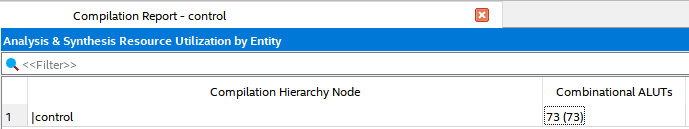
\includegraphics[scale = 0.62]{controltotallogicelement0603.PNG}
    \end{center}
    \caption{Resource Utilization by Entity}
    \label{controltotallogicelement0603}
\end{figure}

\begin{figure}[H]
    \begin{center}
    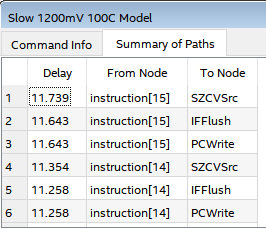
\includegraphics[scale = 1.2]{controlreportpath.PNG}
    \end{center}
    \caption{Report Path...の結果}
    \label{controlreportpath}
\end{figure}


\subsection{ハザード検出ユニット}
total logic elementは5(図\ref{hazardtotallogicelement0603})、遅延時間は9.108ns(図\ref{hazardreportpath})、クリティカルパスはIDEX\_RegRd[0]からIFIDWrite(図\ref{hazardreportpath})のパスである。

\begin{figure}[H]
    \begin{center}
    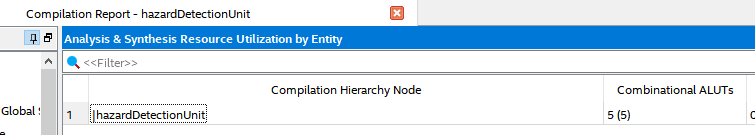
\includegraphics[scale = 0.62]{hazardtotallogicelement0603.PNG}
    \end{center}
    \caption{Resource Utilization by Entityの結果}
    \label{hazardtotallogicelement0603}
\end{figure}

\begin{figure}[H]
    \begin{center}
    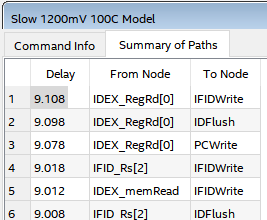
\includegraphics[scale = 1.2]{hazardreportpath.PNG}
    \end{center}
    \caption{Report Path...の結果}
    \label{hazardreportpath}
\end{figure}

\section{考察・感想}
\subsection{考察}
このプロセッサにおいて、実行速度を上げるための考察を記す。このプロセッサは、フォーワーディングにより、WBフェーズからEXフェーズにデータが送られ
、そのデータをALUのオペランドとして使い、SZCVフラグを計算し、そのSZCVフラグをもとに制御部でbranch信号を出力し、それがハザード検出ユニットを通して、IFFlushに入力するパスが、最も長いパスの一つである。SZCVフラグを計算するまでと計算してからで二つのフェーズにわけることで、分岐予測が失敗したときのペナルティは大きくなるかもしれないが、実行可能周波数を大きくでき、実行速度を上げることができるとおもわれる。

\subsection{感想}
五段パイプライン化の構造の設計を主に担当したが、制御部の構造が複雑で特に大変だった。
マルチサイクル方式から、パイプライン化を行うのはそこまで難しくはなかった。SIMPLE/Bの構造を作るのが一番大変だった。
この演習は、各コンポーネントの結合度が強く、分担ができない箇所が多いので、僕のほうが設計の大部分を担い、さらに全体の組み立て、デバックやペアの指導(ペアの理解を助けたり、設計内容や書く内容を指示したり)などもやることになり大変だった。

ただ、プロセッサを作ったことで、プロセッサの構造や、ハザードなどに対する理解が深まり良かったと思う。

\section{実験環境}
実験で使用したボードやCADツールを以下に記す。

\begin{itemize}
\item ボード \\Rapid Prototyping Kit PowerMedusa \\ MU500-RXSET01(MU500-RX, MU500-RK, MU500-7SEG) %\\「」の番号の書かれたボードを使った。  
\item CADツール \\ Quartus Prime Version 17.1.0 Build 590 10/25/2017 SJ Lite Edition
\end{itemize}

\end{document}